           
                %%%%%%%%%%%%%%%%%%%%%%%%%%%%%%%%%%%%%%%%%%%%%%%%%%%%%%%%%%%%%%%%%%%%%%
% LaTeX Template: Curriculum Vitae
%
% Source: http://www.howtotex.com/
% Feel free to distribute this template, but please keep the
% referal to HowToTeX.com.
% Date: July 2011
% 
%%%%%%%%%%%%%%%%%%%%%%%%%%%%%%%%%%%%%%%%%%%%%%%%%%%%%%%%%%%%%%%%%%%%%%
% How to use writeLaTeX: 
%
% You edit the source code here on the left, and the preview on the
% right shows you the result within a few seconds.
%
% Bookmark this page and share the URL with your co-authors. They can
% edit at the same time!
%
% You can upload figures, bibliographies, custom classes and
% styles using the files menu.
%
% If you're new to LaTeX, the wikibook is a great place to start:
% http://en.wikibooks.org/wiki/LaTeX
%
%%%%%%%%%%%%%%%%%%%%%%%%%%%%%%%%%%%%%%%%%%%%%%%%%%%%%%%%%%%%%%%%%%%%%%
\documentclass[paper=a4,fontsize=10pt]{scrartcl} % KOMA-article class
                            
\usepackage[english]{babel}
\usepackage[utf8x]{inputenc}
\usepackage[protrusion=true,expansion=true]{microtype}
\usepackage{amsmath,amsfonts,amsthm}     % Math packages
\usepackage{graphicx}                    % Enable pdflatex
\usepackage[svgnames]{xcolor}            % Colors by their 'svgnames'
\usepackage{geometry}
    \textheight=700px                    % Saving trees ;-)
\usepackage{url}
\usepackage{hyperref}
%\usepackage{times}
\renewcommand{\familydefault}{\sfdefault}
\frenchspacing              % Better looking spacings after periods
\pagestyle{empty}           % No pagenumbers/headers/footers

%%% Custom sectioning (sectsty package)
%%% ------------------------------------------------------------
\usepackage{sectsty}

\sectionfont{%                      % Change font of \section command
    \usefont{OT1}{phv}{b}{n}%       % bch-b-n: CharterBT-Bold font
    \sectionrule{0pt}{0pt}{-5pt}{3pt}}

%%% Macros
%%% ------------------------------------------------------------
\newlength{\spacebox}
\settowidth{\spacebox}{8888888888}          % Box to align text
\newcommand{\sepspace}{\vspace*{1em}}       % Vertical space macro

\newcommand{\MyName}[1]{ % Name
        \Huge \usefont{OT1}{phv}{b}{n} \hfill #1
        \par \normalsize \normalfont}
        
\newcommand{\MySlogan}[1]{ % Slogan (optional)
        \large \usefont{OT1}{phv}{m}{n}\hfill \textit{#1}
        \par \normalsize \normalfont}

\newcommand{\NewPart}[1]{\section*{\uppercase{#1}}}

\newcommand{\PersonalEntry}[2]{
        \noindent\hangindent=2em\hangafter=0 % Indentation
        \parbox{\spacebox}{        % Box to align text
        \textit{#1}}               % Entry name (birth, address, etc.)
        \hspace{1.5em} #2 \par}    % Entry value

\newcommand{\SkillsEntry}[2]{      % Same as \PersonalEntry
        \noindent\hangindent=2em\hangafter=0 % Indentation
        \parbox{\spacebox}{        % Box to align text
        \textit{#1}}               % Entry name (birth, address, etc.)
        \hspace{1.5em} #2 \par}    % Entry value    
        
\newcommand{\EducationEntry}[4]{
        \noindent \textbf{#1} \hfill      % Study
        \colorbox{Black}{%
            \parbox{6em}{%
            \hfill\color{White}#2}} \par  % Duration
        \noindent \textit{#3} \par        % School
        \noindent\hangindent=2em\hangafter=0 \small #4 % Description
        \normalsize \par}

\newcommand{\WorkEntry}[4]{               % Same as \EducationEntry
        \noindent \textbf{#1} \hfill      % Jobname
        \colorbox{Black}{\color{White}#2} \par  % Duration
        \noindent \textit{#3} \par              % Company
        \noindent\hangindent=2em\hangafter=0 \small #4 % Description
        \normalsize \par}

%%% Begin Document
%%% ------------------------------------------------------------
\begin{document}
% you can upload a photo and include it here...
%\begin{wrapfigure}{l}{0.5\textwidth}
%   \vspace*{-2em}
%       \includegraphics[width=0.15\textwidth]{photo}
%\end{wrapfigure}

%\smash{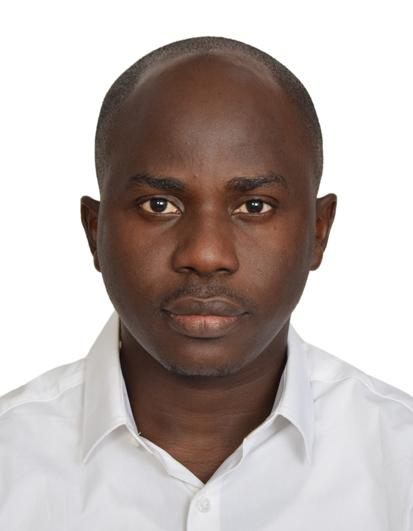
\includegraphics[width=3cm]{images/passport}}

\MyName{Olumide Michael Oyalola}
\MySlogan{Resume}

\smash{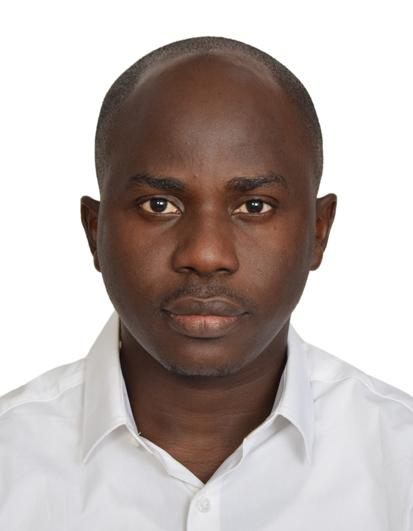
\includegraphics[width=3cm]{images/passport}}


\sepspace

%%% Personal details
%%% ------------------------------------------------------------
\NewPart{Personal details}{}

%\PersonalEntry{Birth}{January 1, 1980}
\PersonalEntry{Address}{69B, Olosan Layout, Alakia, Ibadan, Oyo State.}
%\PersonalEntry{Town/City}{Alakia/Ibadan}
%\PersonalEntry{State}{Oyo State}
\PersonalEntry{Country}{Nigeria}
\PersonalEntry{Phone}{(+234) 803-569-4053}
\PersonalEntry{Skype}{olummyanucitee}
\PersonalEntry{Mail}{\href{mailto:olumideoyalola.at.gmail.dot.com}{olumideoyalola\mbox{}@\mbox{}gmail.com}}
\PersonalEntry{Linkedln}{\href{https://www.linkedin.com/in/olumide-michael-oyalola-9a522857/}{Olumide Michael Oyalola}}
  

%%% Education
%%% ------------------------------------------------------------
\NewPart{Education}{}

\EducationEntry{MSc. Statistics}{2013- 2015}{University of Ibadan, Ibadan, Oyo State, Nigeria}{\textit{\textbf{Modules Completed:} Advanced Probability Theory, Advanced Statistical Inference, Advanced Sample Survey, Advanced Econometrics, Advanced Non-Parametric, Bayesian Statistics, Advanced Time Series.}}
\sepspace

\EducationEntry{B.Tech. Industrial Mathematics}{2005- 2010}{Federal University of Technology, Akure, Ondo State, Nigeria}{\textit{\textbf{Award:} Special Award of Excellence for branding the Federal University of Technology,
	Akure by the Vice Chancellor.}}

%%% Work experience
%%% ------------------------------------------------------------

\NewPart{Work experience}{}

\EducationEntry{Business Transformation Manager}{2019- Present}{Longbridge Technologies Limited, Full time}{
	\begin{itemize}
		\item Work in a cross-functional environment with various business groups, and end-users to identify, document, and communicate business processes.
		\item Create a system to evaluate the success of any adjustments made within the organization and present findings.
		\item Communicate strategies and objectives with relevant departments and colleagues.
		
\end{itemize}}
\sepspace



\EducationEntry{Data Analytics Faculty Member}{2018- Present}{BNet Learning, Part time}{
\begin{itemize}
	\item Designed individualized curricula based on the participants' career path.
\end{itemize}}
\sepspace


\EducationEntry{Freelance Data Science/ Data Analytics}{2018- Present}{Codementor, Part time}{
	\begin{itemize}
		\item	Supports clients through a live session mentoring on task relating to analytic, predictive modeling and statistical programming using R and other related analytical software packages.
\end{itemize}}
\sepspace

\EducationEntry{Data Science}{2017- 2018}{eHealth Systems Africa, Full time}{
	\begin{itemize}
		\item	Developed models to discover the patterns and information in vast amounts of spatial and non-spatial data across several programs at eHA to support better programmatic decisions, intervention planning and improved information products.
		\item	Applied data mining techniques, performed statistical analysis, and build high quality prediction models that formed core of eHA's information products on disease surveillance in particular.
		
\end{itemize}}
\sepspace

\EducationEntry{Data Science}{2016- 2017}{Venture Garden Group Limited, Full-time}{
	\begin{itemize}
\item	Lead discovery processes with Institute stakeholders to identify the business requirements and the expected outcome.
\item	Conducted advanced data analysis and complex designs algorithm.
	\item Applied advanced statistical and predictive modeling techniques to build, maintain, and improve on multiple real-time decision systems.
\item 	Validates analysis using scenario modeling.
	\end{itemize}}
\sepspace

\EducationEntry{Guest Faculty - Business Analytics}{2015- Present}{EduPristine, Part-time}{
	\begin{itemize}
		\item Designed individualized curricula based on the participants' career path.
	\end{itemize}}
	
\sepspace


\EducationEntry{Quality Assurance \& Metrics Analyst}{2013- 2016}{Computer Warehouse Group Plc, Full-time}{
	\begin{itemize}
	\item	Encouraged factual approach to decision making by providing the management an accurate analysis of people and processes.
		\item 	Achieved success in providing standard value-added metrics for business model.
	%	\item Managed the Management Information Dashboard.
	\item 	Continual implementation and auditing of ISO 9001:2008.
	\item 	Quality process analysis to achieving a system thinking organization.
		\item Quality spot checks of project implementations \& Services (Software, Hardware, Communication).
	\item 	Trained a number of employees in HR related work especially Analytics, HSE and Change Management.
		\item Provided both administrative and analytic support to departments in order to manage critical and people sensitive projects.
	\item Collaborated with the VP of Sales in the development of sales forecasts and projections. 
	\item Summarize and report performance against sales quotas to all sales personnel in a timely manner. 
\item 	Proactively prepare and deliver ad hoc customer analysis to sales team members and senior management
	\end{itemize}}

\sepspace


\EducationEntry{Data Analyst}{2012- 2013}{Practical Sampling International Limited, Full-time}{
	\begin{itemize}
		\item Supervised the data collection process of many high profile projects.
		\item Processed and analyzed raw data collected from field work.
		\item 	Improved the statistical procedure usage and reporting method.
	\end{itemize}}


\sepspace


\EducationEntry{Guest Faculty -IBM SPSS\footnote{SPSS: Statistical Package for Social Sciences}}{2011- 2012}{AfriHUB Nigeria Limited, MOUAU, Abia State, Part-time}{
	\begin{itemize}
		\item Improved the knowledge of both students and lecturers of Michael Okpara University of Agriculture, Umudike, Abia State in the usage of statistical software (SPSS) for data analysis.
		\item Designed an electronic test to monitor performance and understanding.
		\item Designed individualized curricula.
	\end{itemize}}






%%% Skills
%%% ------------------------------------------------------------
\NewPart{Skills}{}

\SkillsEntry{Languages}{English (fluent)}
%\SkillsEntry{}{French (Beginner)}
%\SkillsEntry{}{German (fluent)}

\SkillsEntry{Apps/Languages}{Excel, \LaTeX, Apache Spark, \textsc{R}, Apache Hadoop, Python, SQL, ELK}

\SkillsEntry{Tools}{RStudio, Jupyter, Apache Zeppelin, Tableau, Power BI, PostgreSQL}
\SkillsEntry{Environment}{Windows, Linux (Ubuntu, CentOS)}



%%% References
%%% ------------------------------------------------------------
\NewPart{References}{}
Available upon request
\end{document}
